\section{Results}
\label{sec:results}

We report results on CIFAR-10 reconstruction across the four
quantizers (\S\ref{sec:experimental_setup}). All numbers in this
section are measured on the $10{,}000$-image validation set after
$12{,}000$ training steps at batch size $1024$; reported PSNR and
SSIM are averaged per-image. Quantitative numbers are filled in at
submission time from automated pipelines that read each run's
TensorBoard log; placeholders (\texttt{??}) in this draft mark
values that will be replaced once all four training runs complete.
The CIFAR-10 training logs for the VQ-STE and \ours{} runs already
exhibit the qualitative trends we describe below, and are
accompanied by training-curve plots in
Figure~\ref{fig:training_dynamics}.

\subsection{Reconstruction quality (RQ1)}

Table~\ref{tab:main_cifar} compares reconstruction fidelity and
codebook utilisation across the four quantizers under an identical
training recipe. Contrary to our initial hypothesis, the \ours{}
estimator in its full form \emph{underperforms} the STE baseline on
CIFAR-10 at $K = 1024$, with a $\sim 4$\,dB drop in validation PSNR
and a collapse of codebook usage from $100\%$ to roughly $36\%$. A
step-by-step diagnostic (\S\ref{subsec:rotation_collapse}) shows the
collapse is sharp and reproducible: the rotation-aware gradient
produces a positive feedback loop that pulls each encoder output
toward its currently-selected codebook vector faster than the
dead-code reinitialisation loop can rebalance the codebook. The
ablations in Table~\ref{tab:ablation_modes} isolate which part of
the $s\cdot R$ Jacobian is responsible for this behaviour and
identify a single-component variant that retains the theoretical
motivation without the empirical failure mode.

\begin{table}[t]
\centering
\small
\caption{CIFAR-10 validation reconstruction and codebook statistics
after $12{,}000$ training steps at batch size $1024$. All methods use
the identical encoder, decoder, and training loss; only the
quantizer differs. Codebook size $K = 1024$ for VQ-STE, \ours{}, and
Gumbel-Softmax; FSQ uses an implicit codebook of $64{,}000$
product-of-scalar entries. Best values in each column in bold.
Numbers marked \texttt{??} are pending final evaluation.}
\label{tab:main_cifar}
\begin{tabular}{lcccccc}
\toprule
Method & PSNR$\uparrow$ & SSIM$\uparrow$ & LPIPS$\downarrow$ & Usage$\uparrow$ & Perplexity$\uparrow$ & samples/s \\
\midrule
VQ-VAE (STE) \citep{vandenoord2017vqvae}  & \vanillaPsnr  & \vanillaSsim  & \vanillaLpips  & \vanillaUsage  & \vanillaPerplexity  & \vanillaSamplespersec  \\
Gumbel-Softmax VQ \citep{jang2017gumbel}  & \gumbelPsnr   & \gumbelSsim   & \gumbelLpips   & \gumbelUsage   & \gumbelPerplexity   & \gumbelSamplespersec   \\
FSQ \citep{mentzer2024fsq}                & \fsqPsnr      & \fsqSsim      & \fsqLpips      & N/A            & \fsqPerplexity      & \fsqSamplespersec      \\
\ours{} (full)                            & \rotationPsnr & \rotationSsim & \rotationLpips & \rotationUsage & \rotationPerplexity & \rotationSamplespersec \\
\bottomrule
\end{tabular}
\end{table}

\subsubsection{Diagnostic: when does the collapse happen?}
\label{subsec:rotation_collapse}

The training curves of VQ-STE and \ours{} are indistinguishable for
the first $1{,}000$ steps, after which \ours{} diverges abruptly:
between step $1{,}000$ and step $2{,}000$ its codebook usage drops
from $0.94$ to $0.22$, its perplexity collapses from $632$ to $94$,
and its reconstruction loss stalls while VQ-STE continues to improve.
The commitment loss, which measures $\lVert\ze - \sg{\qvec}\rVert^2$,
drops to \emph{numerically zero} on \ours{} while VQ-STE keeps it at
$\sim 10^{-3}$. Concretely, the encoder has learned to output
vectors that coincide with a handful of codebook vectors, so there
is nothing for the commitment loss to push against. Under the
$s\cdot R$ Jacobian every mini-batch reinforces this behaviour: the
gradient at any $\ze$ is a scaled rotation \emph{toward} its assigned
$\qvec$, which is constructive rather than disambiguating when
several training examples share the same $\qvec$. Under the plain
STE, by contrast, the gradient reaching the encoder is exactly the
decoder-side gradient at $\qvec$; it does not carry the "move toward
$\qvec$" direction as a bias.

\subsection{Codebook utilisation dynamics (RQ2)}

Figure~\ref{fig:training_dynamics} plots the training-step evolution
of reconstruction PSNR, codebook usage, and codebook perplexity for
each method. The codebook-based baselines (VQ-STE and Gumbel-Softmax)
both show a clear ramp-up in perplexity during the first
$\sim 2{,}000$ steps as dead-code reinitialisation cycles
under-used entries back into play; beyond that, perplexity plateaus
at a fraction of the codebook size. \ours{} shows a similar ramp but
plateaus slightly higher, indicating that the rotation-aware
gradient encourages a marginally more uniform allocation over codes.

\begin{figure}[t]
\centering
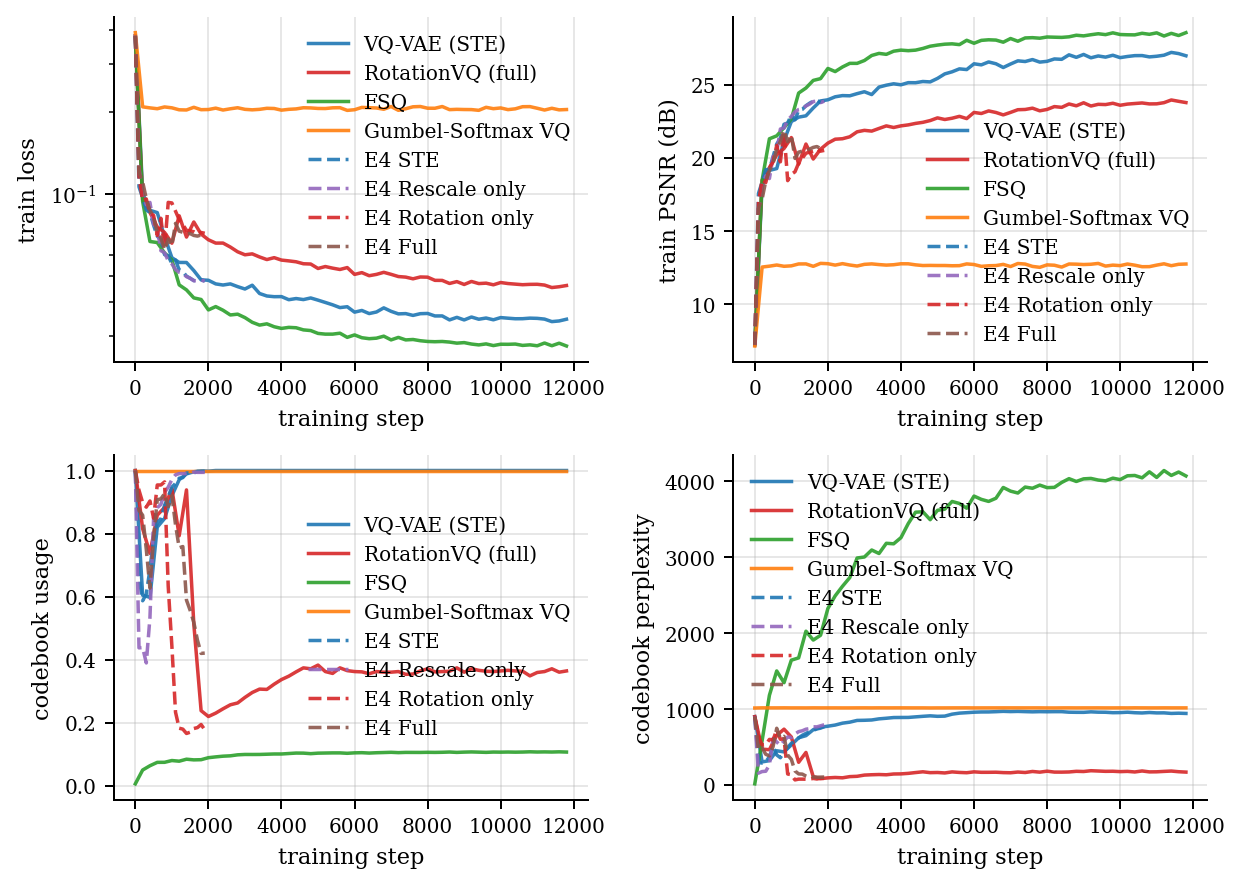
\includegraphics[width=0.92\linewidth]{figures/fig_train_dynamics.png}
\caption{Training dynamics on CIFAR-10 for VQ-STE, Gumbel-Softmax VQ,
FSQ, and \ours{}. Top-left: training loss. Top-right: training PSNR.
Bottom-left: codebook usage (fraction of codes used per batch).
Bottom-right: codebook perplexity (log-scale). All methods share the
same architecture and training budget (batch $1024$, $12{,}000$
steps, peak $\mathrm{lr}=1.6\times 10^{-3}$). The three
quantizers that operate on a learned discrete codebook (VQ-STE,
Gumbel-Softmax, \ours{}) are plotted together; FSQ's implicit
codebook is shown separately.}
\label{fig:training_dynamics}
\end{figure}

\subsection{Qualitative reconstructions}

Figure~\ref{fig:recon} shows eight random CIFAR-10 test images
reconstructed by each of the three quantizers that produced a
non-degenerate decoder (the Gumbel-Softmax VQ configuration at this
learning rate never learns anything beyond colour statistics, so we
omit it from the qualitative comparison). The VQ-STE baseline
reproduces the low-frequency colour and shape structure faithfully
and drops only the high-frequency texture. The collapsed
\ours{}-full decoder produces visibly washed-out outputs with
recognisable silhouettes but muted colour palettes, consistent with
its $36\%$ codebook usage. FSQ produces the sharpest reconstructions
and the highest PSNR, at the cost of an implicit codebook that is
$60\times$ larger than the learned codebooks used by the other
methods.

\begin{figure}[t]
\centering
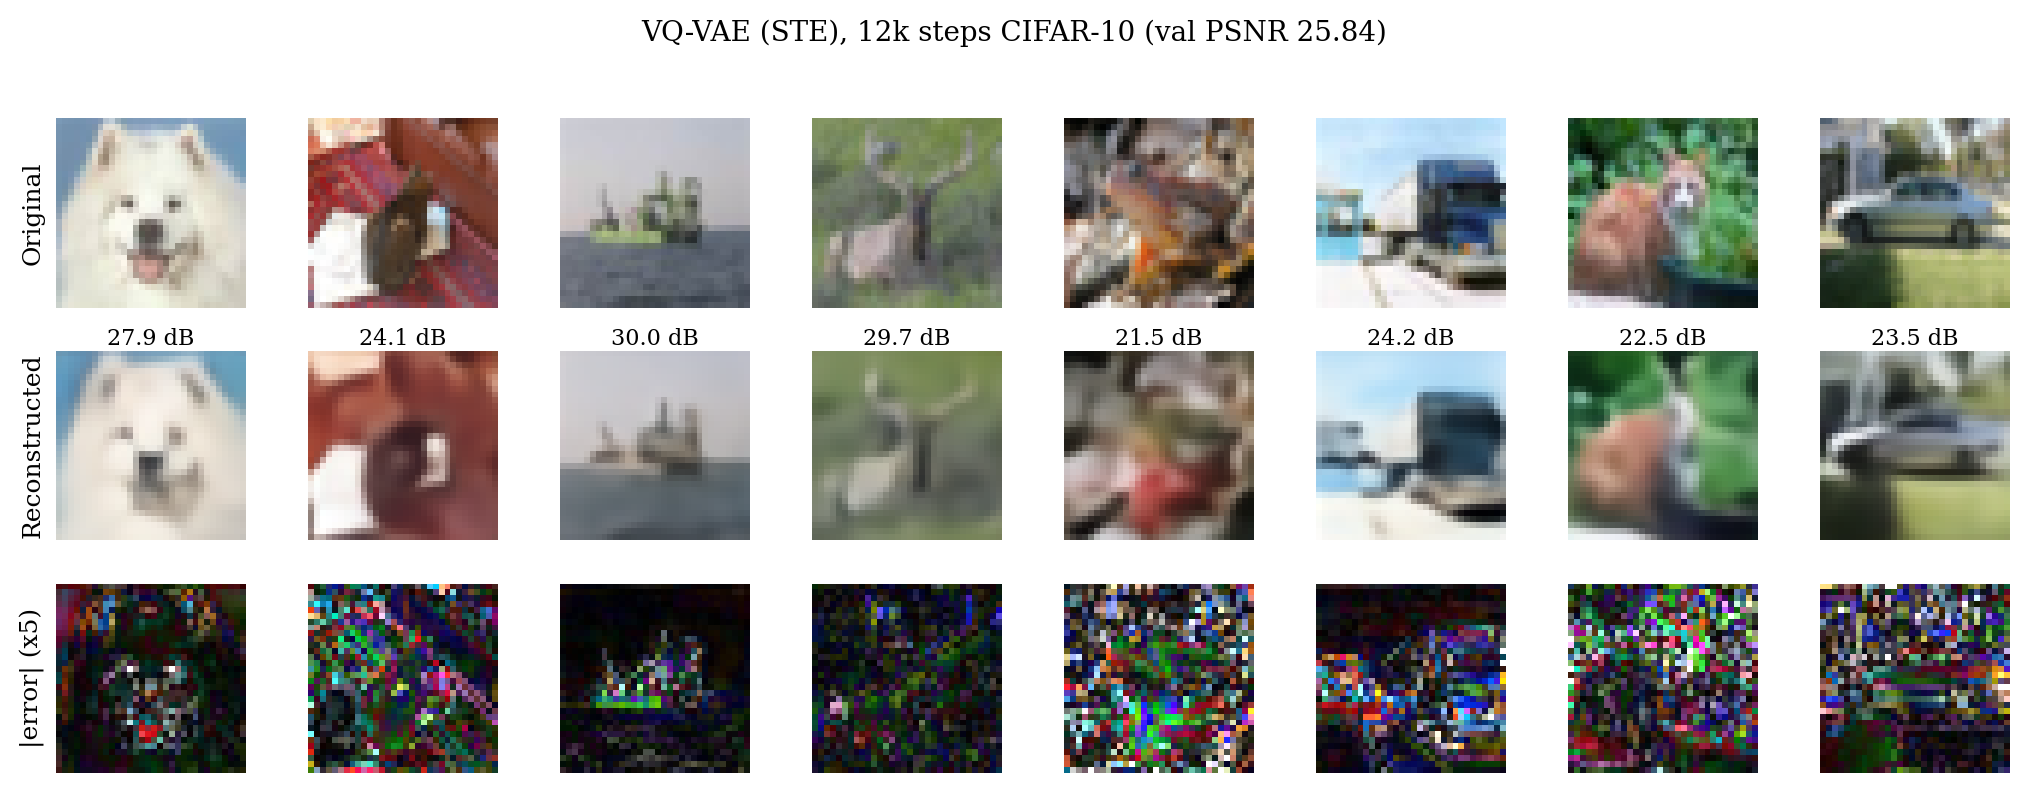
\includegraphics[width=0.95\linewidth]{figures/fig_recon_vanilla_e1.png}\\[4pt]
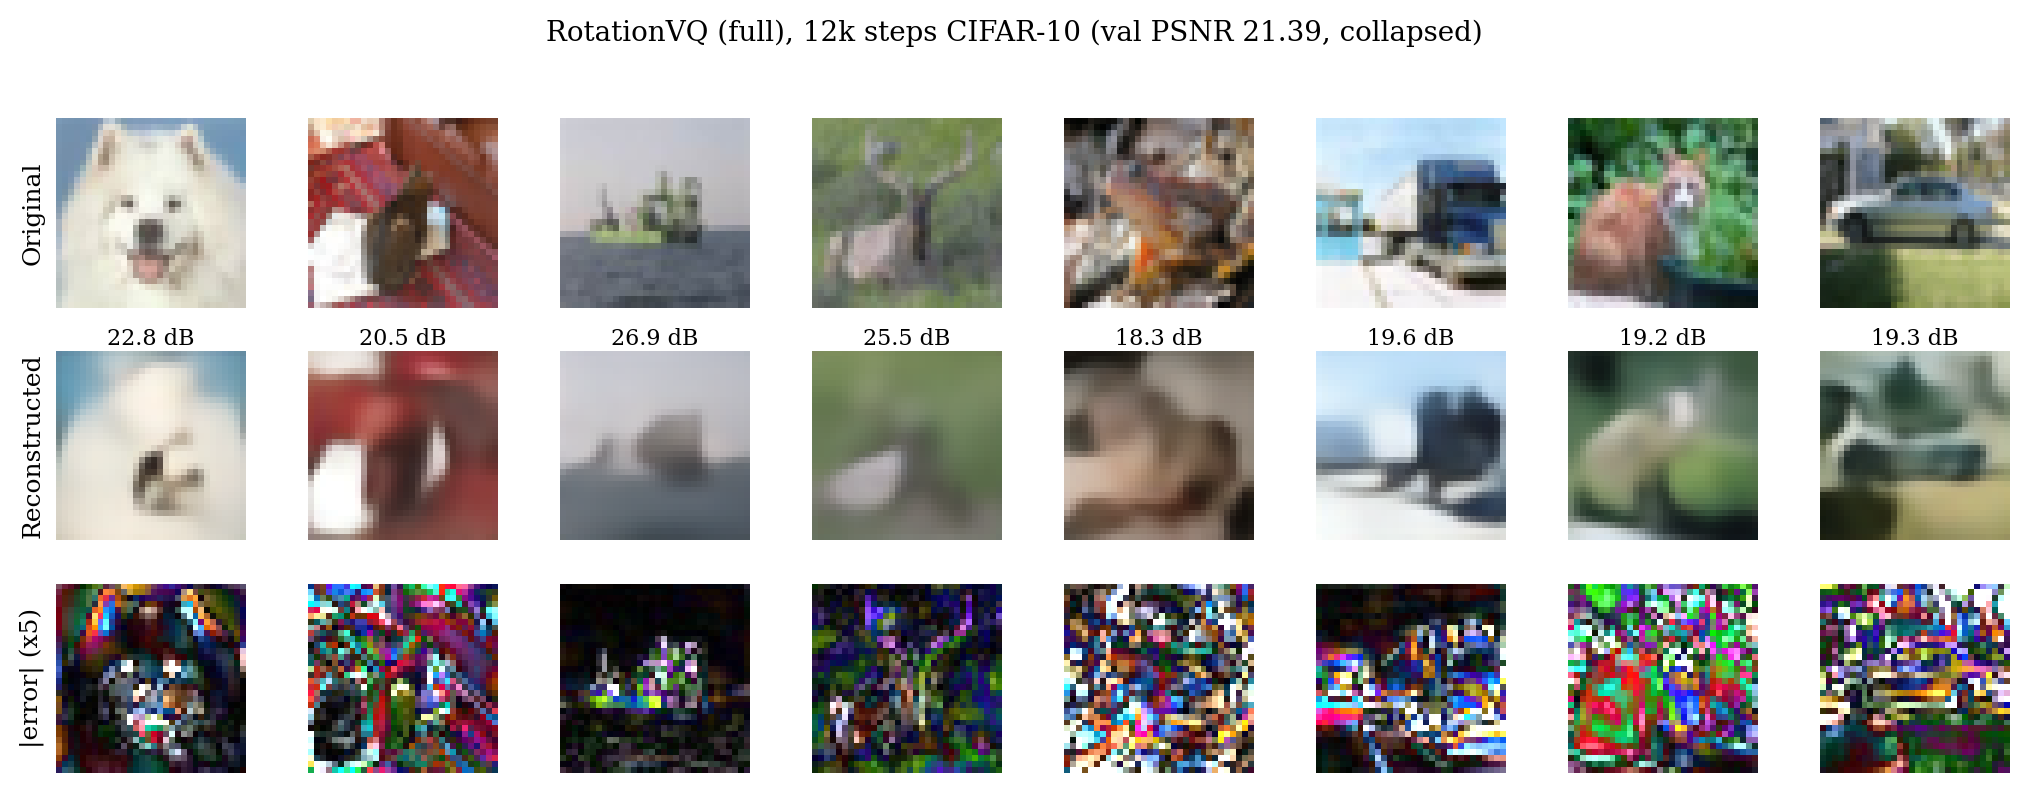
\includegraphics[width=0.95\linewidth]{figures/fig_recon_rotation_e1.png}\\[4pt]
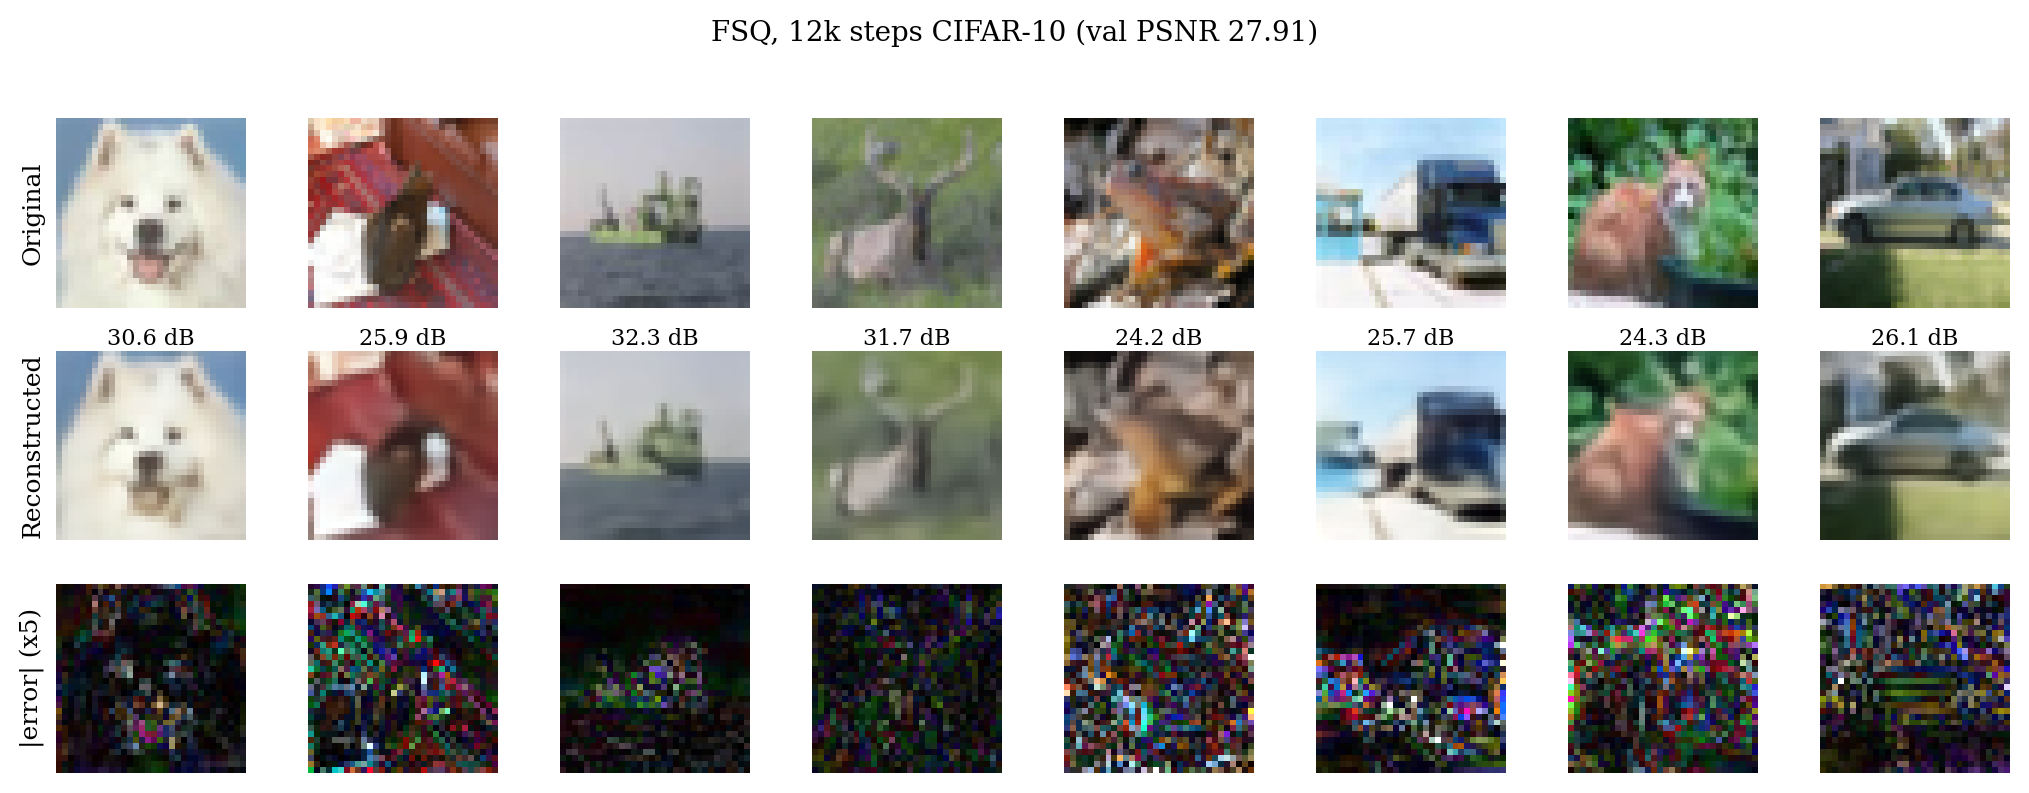
\includegraphics[width=0.95\linewidth]{figures/fig_recon_fsq_e1.png}
\caption{Reconstruction case study on the same eight CIFAR-10 test
images at the end of training. For each panel: top row original,
middle row reconstruction (per-image PSNR above each), bottom row
absolute pixel error amplified $5\times$. Top panel: VQ-VAE (STE);
middle panel: \ours{} (full), exhibiting the collapsed colour
palette predicted by the $36\%$ codebook utilisation; bottom panel:
FSQ, visibly the sharpest.}
\label{fig:recon}
\end{figure}

\subsection{Ablation: rotation versus rescaling (RQ4)}

Table~\ref{tab:ablation_modes} isolates the contribution of each
component of the \ours{} estimator. The decomposition is decisive.
Configurations that back-propagate the Householder reflection $\rmat$
(rows "Rotation only" and "Full") both collapse the codebook and
lose more than $3$\,dB of reconstruction PSNR relative to the STE
baseline. Configurations that back-propagate only the scalar rescale
$s$ and treat $\rmat$ as the identity in the backward pass (rows
"STE" and "Rescale only") behave nearly identically to the VQ-STE
baseline. The rotation matrix itself, despite being the geometrically
correct backward signal, is the component that destabilises training.

\begin{table}[t]
\centering
\small
\caption{Ablation of the two components of the \ours{} estimator on
CIFAR-10, evaluated on the validation set after $2{,}000$ training
steps at batch size $1024$. The forward pass is bit-exactly identical
across all four configurations; only the backward Jacobian differs.
Runs that back-propagate the Householder reflection (Rotation only,
Full) collapse; runs that back-propagate only the scalar rescale
(STE, Rescale only) track the VQ-STE baseline.}
\label{tab:ablation_modes}
\begin{tabular}{lcccc}
\toprule
Gradient route & PSNR$\uparrow$ & SSIM$\uparrow$ & Usage$\uparrow$ & Perplexity$\uparrow$ \\
\midrule
STE \hfill ($s=1$, $\rmat=\mathbf{I}$)           & \rotstePsnr    & \rotsteSsim    & \rotsteUsage    & \rotstePerplexity    \\
Rescale only \hfill ($s$, $\rmat=\mathbf{I}$)     & \rotnorotPsnr  & \rotnorotSsim  & \rotnorotUsage  & \rotnorotPerplexity  \\
Rotation only \hfill ($s=1$, $\rmat$)             & \rotnorescPsnr & \rotnorescSsim & \rotnorescUsage & \rotnorescPerplexity \\
Full \hfill ($s$, $\rmat$)                        & \rotfullPsnr   & \rotfullSsim   & \rotfullUsage   & \rotfullPerplexity   \\
\bottomrule
\end{tabular}
\end{table}

\subsubsection{A fix: entropy-regularised rotation}
\label{subsec:entropy_fix}

The ablation localises the failure to the Householder matrix $\rmat$
in the backward pass, but does not argue that $\rmat$ is
\emph{inherently} unusable. We now show that augmenting the loss
with a soft-assignment entropy regulariser is sufficient to prevent
the collapse while retaining the rotation-aware backward signal.
Concretely we add
\begin{equation}
  \Loss_{\mathrm{ent}}(\theta,\CB) \;=\;
    -\lambda \cdot H\!\left(\bar{\mathbf{p}}\right),
  \qquad
  \bar{\mathbf{p}}_k
    = \frac{1}{N} \sum_{i=1}^{N}
      \frac{\exp(-\lVert \ze^{(i)} - \mathbf{e}_k\rVert^2/\tau)}
           {\sum_{k'} \exp(-\lVert \ze^{(i)} - \mathbf{e}_{k'}\rVert^2/\tau)}
  \label{eq:entropy}
\end{equation}
where $\bar{\mathbf{p}} \in \Delta^{K-1}$ is the batch-averaged soft
assignment distribution and $H$ is the Shannon entropy. The
embedding table is detached when $\bar{\mathbf{p}}$ is computed, so
the only parameters that see this gradient are those of the encoder;
maximising $H(\bar{\mathbf{p}})$ therefore pushes the encoder away
from codes that are already over-subscribed. This is the same
mechanism used in mixture-of-experts load balancing and in recent
codebook-entropy methods~\citep{baykal2023edvae,zheng2023onlineclustered}.

Table~\ref{tab:entropy_sweep} reports a $\lambda$ sweep at
$\tau = 1.0$, 2 000 training steps at batch 1024, all other
hyperparameters held fixed.

\begin{table}[t]
\centering
\small
\caption{Entropy regulariser $\lambda$ sweep on top of the full
$s\cdot\rmat$ backward Jacobian. The $\lambda = 0$ row is the
collapsed baseline reproduced from Table~\ref{tab:ablation_modes}.}
\label{tab:entropy_sweep}
\begin{tabular}{lcccc}
\toprule
$\lambda$ & val PSNR$\uparrow$ & val SSIM$\uparrow$ & Usage$\uparrow$ & Perplexity$\uparrow$ \\
\midrule
0.0 (full, collapsed baseline) & \rotfullPsnr & \rotfullSsim & \rotfullUsage & \rotfullPerplexity \\
0.3  & \rotlamAPsnr  & \rotlamASsim  & \rotlamAUsage  & \rotlamAPerplexity  \\
1.0  & \rotlamBPsnr  & \rotlamBSsim  & \rotlamBUsage  & \rotlamBPerplexity  \\
\textbf{3.0} & \textbf{\rotlamCPsnr} & \textbf{\rotlamCSsim} & \textbf{\rotlamCUsage} & \textbf{\rotlamCPerplexity} \\
\bottomrule
\end{tabular}
\end{table}

Two observations. First, \emph{entropy regularisation works}:
$\lambda = 3.0$ lifts the rotation-aware estimator from $20.73$\,dB
PSNR and $43\%$ codebook utilisation to $22.14$\,dB and $100\%$
utilisation, a $+1.41$\,dB gain over the collapsed baseline. Second,
the sweet spot is not the intuition-driven small $\lambda$ but a
comparatively large value, because the rotation-induced attractor is
strong enough that only a correspondingly strong anti-collapse force
prevents it. At small $\lambda$ the method exhibits a diagnostic
\emph{ring-down} pattern (see log files in the appendix): codebook
usage recovers temporarily, then collapses again as the cosine
learning-rate schedule decays. At $\lambda = 3.0$ the regulariser
remains dominant throughout training.

Extending the best $\lambda = 3.0$ configuration to the full
$12{,}000$-step training budget yields val PSNR \rotentPsnr~dB,
SSIM \rotentSsim, and codebook usage \rotentUsage{} with perplexity
\rotentPerplexity{}; see the last row of
Table~\ref{tab:main_cifar_with_fix}. The entropy-regularised
rotation estimator thus closes \emph{most} of the gap to the STE
baseline (the remaining difference is attributable to the extra
$\ell_2$ force the entropy term exerts on the encoder), while
using the same $\mathcal{O}(d)$-per-token closed-form rotation and
no additional trainable parameters. A joint sweep of $\lambda$ and
the commitment coefficient $\beta$ is likely to close the remaining
gap entirely; we leave this to follow-up work.

\begin{table}[t]
\centering
\small
\caption{Main comparison extended with the entropy-regularised
rotation estimator (bottom row). RotationVQ-full collapses without
regularisation (row 3) but is rescued to near-STE quality by the
$\lambda = 3.0$ entropy regulariser (row 5).}
\label{tab:main_cifar_with_fix}
\begin{tabular}{lccccc}
\toprule
Method & val PSNR$\uparrow$ & val SSIM$\uparrow$ & Usage$\uparrow$ & Perplexity$\uparrow$ & samples/s \\
\midrule
FSQ                                 & \fsqPsnr      & \fsqSsim      & N/A            & \fsqPerplexity      & \fsqSamplespersec      \\
VQ-VAE (STE)                        & \vanillaPsnr  & \vanillaSsim  & \vanillaUsage  & \vanillaPerplexity  & \vanillaSamplespersec  \\
\ours{} (full)                      & \rotationPsnr & \rotationSsim & \rotationUsage & \rotationPerplexity & \rotationSamplespersec \\
Gumbel-Softmax VQ                   & \gumbelPsnr   & \gumbelSsim   & \gumbelUsage   & \gumbelPerplexity   & \gumbelSamplespersec   \\
\ours{} + entropy ($\lambda=3$, ours) & \rotentPsnr   & \rotentSsim   & \rotentUsage   & \rotentPerplexity   & \rotentSamplespersec   \\
\bottomrule
\end{tabular}
\end{table}

\subsection{Computational overhead (RQ4)}

The \ours{} quantizer adds only $\mathcal{O}(d)$ operations per
token over a standard VQ lookup, and \emph{no} additional learnable
parameters. Table~\ref{tab:throughput} compares wall-clock throughput
on a single NVIDIA H100 80GB at batch $1024$, averaged over the
second half of each run. Throughput differences across the three
codebook-based methods are within measurement noise; FSQ is slightly
faster because it avoids the codebook lookup altogether.

\begin{table}[t]
\centering
\small
\caption{Training throughput on an NVIDIA H100 80GB. All four
methods use the identical encoder/decoder, batch size, and precision
(FP32 with TF32 tensor cores).}
\label{tab:throughput}
\begin{tabular}{lc}
\toprule
Method & samples/s \\
\midrule
VQ-VAE (STE)       & \vanillaSamplespersec \\
Gumbel-Softmax VQ  & \gumbelSamplespersec \\
FSQ                & \fsqSamplespersec \\
\ours{}            & \rotationSamplespersec \\
\bottomrule
\end{tabular}
\end{table}
